\chapter{TSP Approximation}
\label{chapter:tsp}

A well-recognized problem in combinatorial optimisation is the Travelling Salesman Problem (TSP). It is usually presented in a practical form: given a list of $n$ cities and distances between them, find the shortest route that visits each city exactly one time and returns to the city of origin \cite{kruskal1956shortest}. The problem is NP-hard and finding solution is not trivial. However, it reflects many practical examples and the ability to quickly solve it is very desirable. Any TSP problem can be converted into QAP, thus TSP can be though as a specialisation of Quadratic Assignment Problem. To do such conversion a TSP distance matrix can be used without any changes as the QAP distance matrix, while a QAP flow matrix is filled with same constant values.

The Physarum-based Metaheuristic that was introduced in this thesis, is a method of looking through the space search and it is not dependant on any specific problem. It can be used with ease for other problems than QAP, however, a definition of the neighbourhood and a cost function is required. As an example, we made simplified tests of the algorithm, approximating TSP tour.


\section*{Implementation}

While any instance of TSP could be treated as an instance of QAP, we preferred to create a specialised implementation of the \texttt{Problem} class, as it needs not to store any flow values. A \texttt{TspProblem} has been created, which defines $cost$ as a sum of distances between each of the cities in the tour. The same neighbourhood as in QAP is used: a single pair swap in a tour, thus creating the neighbourhood of size $\frac{n\cdot(n-1)}{2}$ for every possible tour.

An input format is simpler than with QAP, as only a single matrix needs to be provided --- the first line of the input contains a size of the problem $n$, followed by $n{\times}n$ numbers representing the distance matrix. The output is defined as in QAP --- the problem size $n$, followed by a total distance of the tour $f$, followed by a list of $n$ numbers representing the tour (rearranged so it starts with the city numbered one).

Using \texttt{build.sh} script, the executable files \texttt{bin/physarum-tsp} and \texttt{bin/physarum-tsp-debug} can be created. The configuration options are the same as with QAP version (table \ref{table:pi_options}).


\section*{Results}

The test dataset is a subset of TSPLIB, which is a library containing multiple instances of synthetic and practical problem definitions with the optimal tours \cite{reinhelt2014tsplib}. The data from the TSPLIB has been preprocessed to be compliant with the input format.

In comparison to QAP usecase, it has been observed that larger values of $E_{explore}$ are preferred (figure \ref{figure:tsp_explore_frontier}). Usage of large values of $E_{explore}$ forces the plasmodium to prefer a deeper crawling than a local exploration. Furthermore, usage of $E_{explore}=0.01$ gives the plasmodium the biggest amount of the energy, even though less solutions are explored (figure \ref{figure:tsp_explore_energy}).



\begin{figure}
  \centering

  \includegraphics[width=1.1\textwidth,center]{algorithm/metaheuristic/charts/tsp/u/tsp_explore_frontier.\eop}

  \caption{Cost of the best detected solution with different exploration energy $E_{explore}$ (dataset \texttt{berlin52})}
  \label{figure:tsp_explore_frontier}
\end{figure}

\begin{figure}
  \centering

  \includegraphics[width=1.1\textwidth,center]{algorithm/metaheuristic/charts/tsp/u/tsp_explore_energy.\eop}

  \caption{Plasmodium energy $E_{plasmodium}$ with different explore energy $E_{explore}$ (dataset \texttt{berlin52}, $q=10$, $a=0.1$)}
  \label{figure:tsp_explore_energy}
\end{figure}

However, it can be seen that usage of the default exponential base $q=10$ and a scaling factor $a=0.1$ in the cost-to-food transformation, makes the energy vary much with each epoch. This is a subefficient behaviour and should be controlled --- providing more energy for a mildly better solution causes the plasmodium to stay longer in a local minima neighbourhood. The neighbourhood in TSP have different characteristics than QAP, even a small change can result in a large change of length of the tour. Different scaling factors have been tested, that showed that rather smaller values of $q$ (and $a=\frac{1}{q}$) are preferred (figure \ref{figure:tsp_ctf_energy}). As a result of choosing smaller values of the exponential base $q$, the algorithm behaves less erratically, which leads to better solutions (figure \ref{figure:tsp_ctf_frontier}).

\begin{figure}
  \centering

  \includegraphics[width=1.1\textwidth,center]{algorithm/metaheuristic/charts/tsp/u/tsp_ctf_energy.\eop}

  \caption{Plasmodium energy $E_{plasmodium}$ with different exponential base $q$ (dataset \texttt{berlin52}, $a=\frac{1}{q}$)}
  \label{figure:tsp_ctf_energy}
\end{figure}

\begin{figure}
  \centering

  \includegraphics[width=1.1\textwidth,center]{algorithm/metaheuristic/charts/tsp/u/tsp_ctf_frontier.\eop}

  \caption{Cost of the best detected solution with different exponential base $q$ (dataset \texttt{berlin52}, $a=\frac{1}{q}$)}
  \label{figure:tsp_ctf_frontier}
\end{figure}

Considered TSP instances are rather large, therefore using a large number of initial samples $k$ is recommended (figure \ref{figure:tsp_samples_cost}). The colony of virtual plasmodium is started on better solutions, thus requiring fewer epochs for being close to optimum.

\begin{figure}
  \centering

  \includegraphics[width=1.1\textwidth,center]{algorithm/metaheuristic/charts/tsp/u/tsp_samples_cost.\eop}

  \caption{Cost of the best detected solution with different number of initial samples $k$ (dataset \texttt{berlin52}, $q=1.25$, $a=0.8$, $E_{explore}=0.01$, $l=10$)}
  \label{figure:tsp_samples_cost}
\end{figure}

Even though a rather large values of $E_{explore}$ are preferred for the algorithm's stabilisation, when using a large number of samples $k=1000000$, an initial solution can be quite close to the optimum. Therefore, the thorough exploration of the local neighbourhood could result in finding even better solutions at initial epochs. In order to allow such a behaviour, some initial energy $E_{initial}$ must be introduced, so more exhaustive exploration phase can be done, though the same $E_{explore}$ is used. Selecting a rather large $E_{initial}=100$ allows for exploring extra $10000$ neighbour solutions (when $E_{explore}=0.01$), resulting in better overall results (figure \ref{figure:tsp_initial_cost}).

\begin{figure}
  \centering

  \includegraphics[width=1.1\textwidth,center]{algorithm/metaheuristic/charts/tsp/u/tsp_initial_cost.\eop}

  \caption{Cost of the best detected solution with different initial energy $E_{initial}$ (dataset \texttt{berlin52}, $q=1.25$, $a=0.8$, $E_{explore}=0.01$, $l=10$, $k=1000000$)}
  \label{figure:tsp_initial_cost}
\end{figure}

\section*{Conclusion}

The usage the Physarum-based Metaheuristic to approximate tours of the Travelling Salesman Problem required different tuning of the algorithm as the problem has much different characteristics than QAP. Using the parameters that have been chosen experimentally (a scaling factor $a=0.8$, an exponential base $q=1.25$, $E_{explore}=0.01$, $l=10$, $k=1000000$, $E_{initial}=100.0$, $E_{crawl}=0.001$), tests have been performed on a subset of instances varying in size, that were selected from the \texttt{TSPLIB}. In total tests have been performed ten times for each instance, time limited to $t=10n$, but no longer than 3600~s. Aggregated results in a form of a distance to the optimal length are provided in a figure \ref{figure:tsp_final}.

\begin{figure}
  \centering

  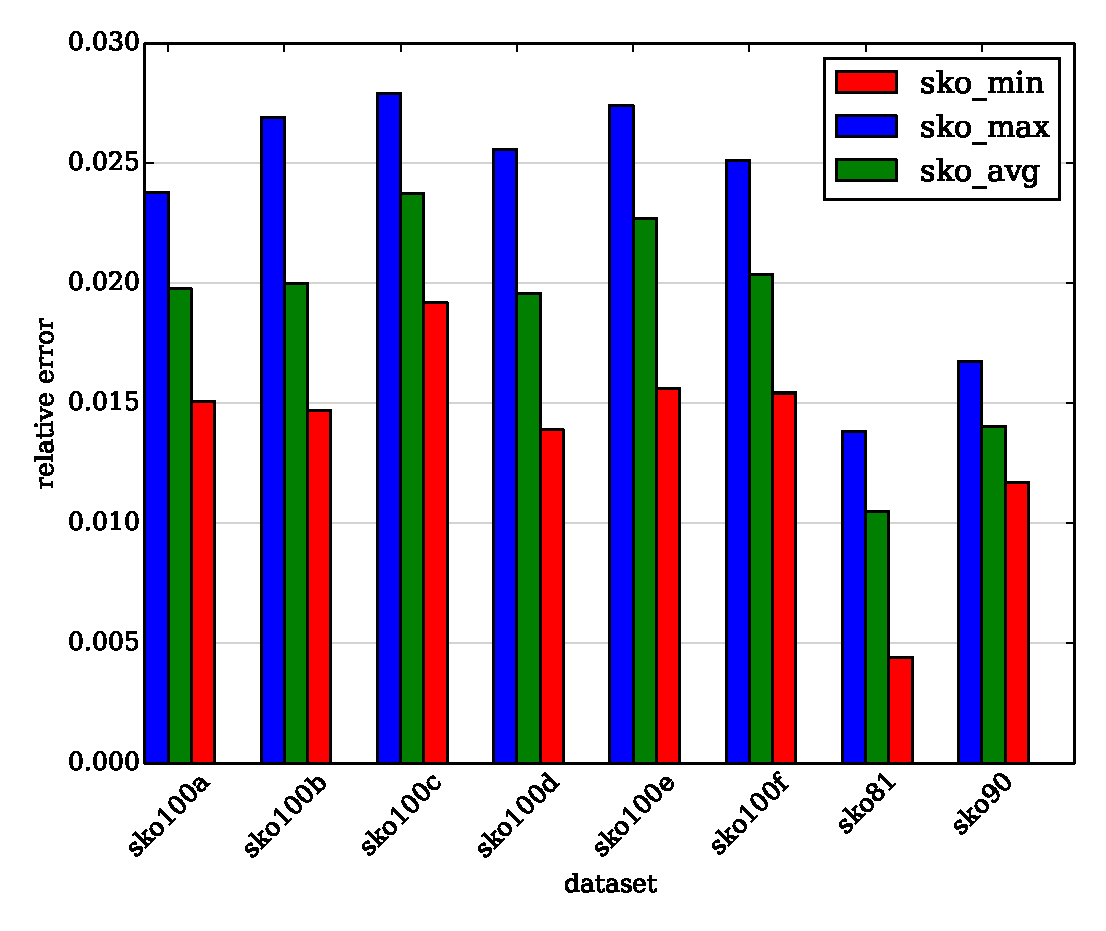
\includegraphics[width=0.9\textwidth]{algorithm/metaheuristic/charts/tsp/final/distance.eps}

  \caption{Aggregated results for various TSP instances}
  \label{figure:tsp_final}
\end{figure}

In the end, it can be seen that proposed algorithm behaves quite well on multiple datasets, yielding results at most $10\%$ worse than optimal tours, however on some datasets approximated tours are far from optimal and cannot be considered useful. Some further work is needed in order to make the results of Physarum-based Metaheuristic reliable approximations of the TSP tours.
